\section{主要内容}

标题:硬件比软件更安全吗?

作者: Lianying Zhao | Carleton University,David Lie | University of Toronto

文章内容:计算机硬件通常被认为比软件更安全。然而,最近的趋势使我们重新审视这一信念。我们应该注意到硬件的“稳固化”,并主张重新审视硬件和软件在系统安全中的作用。

通常来说,计算机系统可以看作是由两种部件组成:硬件和软件。硬件是指执行一组固定操作的物理组件。另一方面,软件定义逻辑元素,逻辑元素被实例化为数据和指令,可以指定硬件操作的任意序列以及这些进程的输入。一个功能可以使用各种硬件和软件组件(甚至完全在硬件中)来实现。硬件和软件的混合可能会对功能执行的某些属性产生影响(例如,性能和安全性)。

\begin{tcolorbox}[title={个人理解}]
    因此,这里指出了带来安全或性能上影响的原因是软件与硬件的混合使用。
\end{tcolorbox}

\subsection{硬件安全性}

数十年来,硬件一直被认为是安全敏感操作的保障。这反映在硬件安全模块(HSM)的长期使用中,例如用于密码处理的防篡改/防篡改IBM加密卡,以及最近对使用可信计算技术保护敏感任务的研究兴趣,如Intel Software Guard Extensions(SGX)和ARM TrustZone。

在学术界,硬件安全也引起了研究人员的极大关注。在Google Scholar上快速搜索,截至本文撰写时,至少有1750份学术出版物的标题同时包含“hardware”和“security”。

虽然这是对此类出版物实际数量的一个保守的下限估计(因为搜索仅检查标题),无论它们是否建议硬件在安全方面发挥更大的作用,还是试图检查硬件对安全攻击的脆弱性,这一庞大的数字非正式地说明了安全团体对计算机硬件和安全之间的关系有着强烈的兴趣。另一个最近的趋势是实现硬件机制来解决众所周知的安全问题。例如,一项调查列出了21种基于硬件的体系结构,以确保控制流的(正确性)完整性,这是程序的正确执行顺序。这意味着人们有一个基本的信念,即硬件实现与计算系统中更好的安全属性有很强的关联性。

\subsection{硬件的安全优势}

我们首先要检查这种对硬件安全好处的信念是从何而来的。直觉上,人们可能会认为安全感可能源于拥有和实际存在的硬件。硬件开关提供了操作完整性的可见保证;例如,设置了一个状态,并且它是可以轻松观察到的。类似地,用户可以确信他们拥有并控制可拆卸设备(如USB加密和驱动器)固有的信息和功能。在第一次检查中,硬件部件比许多软件元件更简单,功能更受限制。像硬盘这样的组件存储数据,而键盘提供了一种输入信息和命令的手段。事实上,硬件的物理特性意味着在将组件运送给客户之后,缺陷就不那么容易修复了,这促使硬件设计师更加保守和体贴。与软件相比,所有这些特性都有助于在硬件方面获得更好的安全性和可靠性。

\begin{tcolorbox}[title={个人理解}]
    因为硬件看上去限制更多,因此在出厂送到用户之前,就会经过大量的测试,安全性或是性能上,这样给用户一种安全性。这种假设是,硬件开发者比软件开发者更有责任心,设计得更加完备。
\end{tcolorbox}
然而,如果我们抛开对硬件和软件设计者的责任心的假设,以及对物理组件和逻辑组件可能存在的心理偏见,而是关注从安全角度区分硬件和软件实现的功能属性,我们可以指出两个方面似乎突出:不变性和特权。我们将不变性定义为一个功能的属性,描述了其抵抗改变其最初设计的能力。因为硬件在物理上是在电路和晶体管中实现的,所以它具有“内在”的不变性:在硬件中实现的功能不能简单地通过改变内存中的一些位来改变。如果攻击者想要修改硬件的功能,他或她必须对其进行实质性的更改,这意味着需要对受害者进行人身访问。这是令人欣慰的,因为物理变化更容易留下篡改的痕迹。

这种不变性也可以被认为是硬件不需要实现“图灵机器”这一事实的好处。硬件对“机制的经济性”有一种固有的偏见[10]。因为它有物理实体存在,额外或未使用的功能会受到惩罚(损失),因此有强烈的动机来避免多余的功能。因此,硬件逻辑通常只实现足够的功能来执行指定的任务而不启用任意操作。这种天然的缺陷限制了用硬件来做危害:电路中的硬件开关可能被恶意地从关闭更改为打开,但不能重新编程来做一些本质上不同的东西。相反,软件通常运行在一个图灵完备的执行引擎上(比如CPU),其可以被编程来做一些与其设计出来完全不同的功能。因此,如果受到破坏或有缺陷,软件可能会从本质上让攻击者访问图灵完全环境,在那里可以执行随机(任意)功能。

我们将特权定义为观察和控制另一个组件的操作的能力。这一定义与特权的软件特征(即内核与用户)有细微的区别,因为高权限软件通常能够对低权限软件进行超集操作。然而,硬件相对于软件的特权是不同的,因为硬件和软件不具备相同的进程集。然而,授权是可比较的,因为特权软件执行的附加功能通常包括控制(即,启动、停止和中断)和观察(读写)非特权软件的执行状态的能力。同样地,构成软件执行引擎的硬件具有同样的能力来控制和观察它运行的任何程序的状态。

\begin{figure}[!h]
    \centering
    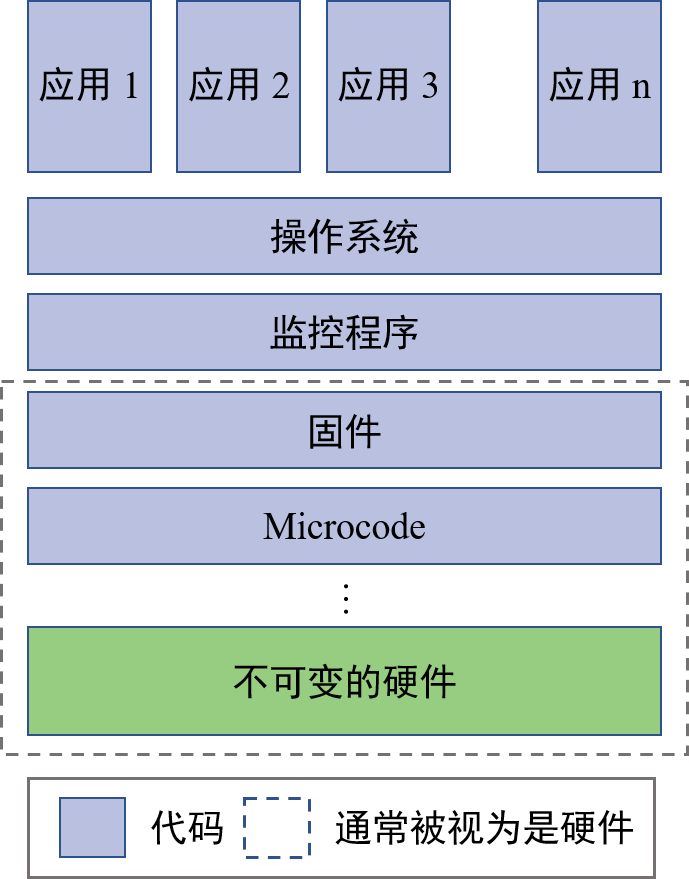
\includegraphics[width=0.75\linewidth]{ise3-fig1.png}
    \caption{现代计算机系统中的分层结构}
    \label{fig:layers}
\end{figure}

现代计算机都采用一种分层结构,从硬件/固件、虚拟机管理程序和操作系统(OS)开始,扩展到应用程序(见图\ref{fig:layers})。hypervisor针对OS内核是安全的,而OS内核又是针对应用程序的安全的。在这个堆栈中,硬件处于最特权的位置,因此可以自然地防止低特权软件层中的漏洞和来自低特权软件层的攻击。

\subsection{硬件、固件和软件}

至此,我们讨论了一个计算机系统的高层抽象模型,包含了整个软件和硬件。然而,正如读者可能已经猜到的那样,本文提出的计算系统的观点并不是那么简单。实际上存在第三种,混合类型的计算功能实现,它被称为固件。“固件”一词几乎和计算机硬件存在的时间一样长;它是由Ascher Opler4在20世纪60年代提出的。固件与软件有一些共同的属性,因为它是作为在通用图灵完整硬件处理器上执行的软件指令来实现的。为了更好地理解硬件、固件和软件,我们使用四个属性对三者进行比较:不变性、特权、效率和成本;表\ref{tab:prop}总结了它们。

\begin{table}[h]
    \centering
    \caption{硬件、固件和软件的性质对比}
    \begin{tabular}{l|l|l|l}
        \toprule
        性质     & 硬件       & 固件     & 软件     \\
        \midrule
        不可变性 & \checkmark & $\times$ & $\times$ \\
        \hline
        特权     & 最高       & 中等     & 低       \\
        \hline
        效率     & 高         & 中等     & 低       \\
        \hline
        成本     & 高         & 低       & 低       \\
        \bottomrule
    \end{tabular}
    \label{tab:prop}
\end{table}

\begin{enumerate}
    \item  \textbf{不变性}:如前所述,不变性表征组件的功能是否可以更改。虽然硬件的不变性是固有的,但固件和软件的不变性不是,而且它通常必须由其他组件(硬件或软件)强制执行。例如,固件的地址空间通常被应用程序阻止访问,在许多情况下,甚至操作系统被硬件参考监视器或硬件和软件参考监视器的某种组合所阻止。由此,我们认为只有硬件才是真正不变的,而固件和软件可以被某些组件有意地改变,或者由于设计和实现缺陷而可变。在我们的讨论中,我们排除了供应链攻击,因为当产品在用户获得之前就被破坏了,不变性不再适用。即使在这种情况下,受损的硬件仍然是不可变的;例如,设计者或制造商插入的特洛伊木马通常不能被固件/软件删除。

    \item  \textbf{特权}:同样是前面定义的,Privilege表示具有较高权限的组件观察和控制具有较少权限的元素的执行的能力。因为所有的软件都必须在硬件上执行,所以硬件本身就拥有比固件和软件更高的特权。然而,通常情况下,固件存在于硬件-软件接口的硬件端,因此它对软件具有特权,例如操作系统内核和应用程序。因此,我们订购的特权是硬件在顶部,固件在中间,最后是软件在底部。

    \item  \textbf{效率}:这定义了实现作为某种资源(例如电力)的函数所提供的性能。硬件实现通常比软件更省电,并且在相同的能耗下提供更好的性能。虽然固件和软件的效率都不如纯硬件块,但固件的执行通常更接近硬件,并且它可以访问特殊的硬件功能和设施,使其比软件更经济。例如,CPU固件(即微码)不会像常规应用软件那样受到上下文切换和操作系统调度的影响。

    \item \textbf{成本}:一般来说,每个系统的硬件成本是固定的,而为每个系统部署软件的增量成本几乎为零。因此,包含更专业化硬件的系统通常生产成本更高,这意味着最终用户的购买价格更高。这就产生了一个几乎每个计算机工程师都意识到的直观权衡:使用硬件加速器的更快的系统成本更高。
\end{enumerate}

\subsubsection{固件所处的位置}

考虑到表\ref{tab:prop}中的比较,人们可能想知道为什么首先引入固件,因为它似乎在任何属性上都不优于硬件或软件。固件的一个重要原因是,它可以在各种计算机系统接口之间保持互操作性。

简言之,互操作性意味着组件的不同实现可以彼此协作,因为组件都遵循一个标准接口。然而,使用不同的硬件和软件组合来实现该接口,使得制造商能够在不同的成本效率范围内创建不同的产品。例如,所有网卡基本上都执行相同的功能,但是更昂贵、更快的网卡可能包含各种加速器和卸载引擎,这些加速器和卸载引擎有助于更快地处理数据包,从而使用更少的功率,同时释放主CPU上的通用计算周期。类似的例子是专门的加密函数加速器。在某些情况下,不是那么性能敏感的操作都可以通过固件来实现。由于这些变体不影响接口,因此可以在不改变软件或其他硬件组件的情况下互换使用。

固件提供的另一个重要优势是能够更新或修补硬件,以提供增强功能或解决缺陷。从网络摄像头到恒温器和家庭路由器等各种消费设备,其大部分高级功能都是在固件中实现的,因此可以在现场进行更新,为最终用户带来更多价值。事实上,一些智能手机型号的一个关键卖点是,供应商将继续修补固件中的安全漏洞。

\subsection{硬件固件化}

硬件安全的一个关键支柱是对软件的不变性,当硬件实际实现为硬件时,这一点最自然。然而,近年来软硬件的实现越来越与其它硬件有关。随着硬件变得越来越复杂,许多这些复杂的特性实际上是作为固件实现的。

Baumann指出,硬件是新的软件,强调了现代硬件功能实现的快速和迭代方式。许多现代硬件“特性”实际上是作为固件实现的,它们通常是迭代地推出的,即SGX,然后是SGX2。通过改变固件可以修补硬件中的缺陷,而不是实际更换组件。这些特性越来越多地赋予了硬件软件的优点(即灵活性和可升级性)和缺点(复杂性和易变性)。

将硬件和固件视为一个整体都是硬件,这个观点并不少见。如图1所示。例如,诸如“硬件加密的驱动器比软件完整磁盘加密更安全”这样的笼统说法并不能完全承认诸如硬件加密实现通常包含软件(固件)组件这样的细微差别。更糟糕的是,传统上被认为是“哑”的设备(即,不是图灵完备的),当固件丰富(即引入通用处理器)时,就会变成图灵完备的,并且,如果受损,可以执行原始设计中从未打算的功能。键盘就是一个例子,苹果公司的一个设备仅仅通过使用软件工具就变成了一个击键记录器。

\subsection{固件化后的硬件是如何导致错误的}

当使用固件实现硬件功能时,硬件的不变性会受到影响,弱化了面对攻击的安全性。在本节中,我们将检查过去的一些硬件安全故障,并了解如何出现一个常见线程,攻击者会意外地修改固件中实现的功能。我们还将展示固件化及其安全后果如何在不同的计算机组件中普遍存在。在我们的讨论中,我们关注两个方面:漏洞本身,它会导致针对任意代码执行的固件损害,以及该漏洞所造成的危害。实际上,在本节中,我们将研究过去的一些硬件安全故障,并了解如何出现一个常见线程,攻击者会意外地修改固件化中实现的功能。我们还将展示固件化及其安全后果如何在不同的计算机组件中普遍存在。在我们的讨论中,我们关注两个方面:漏洞本身,它会导致针对任意代码执行的固件损害,以及该漏洞所造成的危害。

\subsubsection{输入输出设备}

计算机外围设备,如驱动器、键盘、鼠标和打印机,通常被视为过于简单,不易受到危害,被用于攻击。然而,这些设备已经越来越多地提供了越来越多的功能,这些功能通常是在固件中实现的,从而导致了漏洞。

\textbf{硬盘}。硬盘和固态硬盘,通常被视为简单的块设备,实际上包含了相当多的固件。最近对今天的自加密SSDs6的(in)安全性进行的分析发现,在关键的MX100/MX200上发生了一次仅限软件的固件刷新攻击,该攻击是使用一些未经记录的供应商特定命令(VSC)执行的。此漏洞使攻击者能够远程、秘密地截获任何进出磁盘的数据,而不会在主机上留下痕迹。(我们在这里使用“远程”意味着坏角色不需要物理访问,但可能仍然必须首先在本地操作系统上执行远程权限提升。)与常规恶意软件不同,恶意代码驻留在固件中,因此,即使完整的操作系统重新安装也无法消除感染。2013年,Zaddach等人3证明了隐形后门可以通过软件安装在现成的机械硬盘上。Jeroen Domburg(又名sprite\_tm)也在同年独立发现了这个漏洞。

\textbf{网卡}。除了硬盘,网卡是另外一个向固件化妥协的例子。早在2006/2007年,所谓的Maux Mk.I项目,Triulzi通过修改固件,展示了对Broadcom网卡的部分概念验证接管。2010年,Duflot和Perez利用Broadcom NetXtreme NIC中的漏洞将此攻击扩展到完全控制计算机。该漏洞位于处理警报标准格式协议的固件中,该协议是一个用于远程管理的模糊过程。

\textbf{视频显卡}。显卡还包含一个在名为videobios(VBIOS)的组件中的固件,该组件在CPU上的加载和执行方式与常规系统BIOS的方式大致相同。有人试图调整VBIOS,比如nvsresolution,12它通过帧缓冲驱动程序增加了对更好分辨率的支持。视频卡可以被用来执行恶意代码,从而避开传统的恶意软件检测。图形处理单元(GPU)和视频随机存取存储器(RAM)为恶意软件提供了一个完整的执行环境,与CPU共享的内存可以发动攻击。例如,在2013年,研究人员实现了一个基于GPU的键盘记录器,它可以窥视通常由CPU管理的键盘缓冲区。

\textbf{其他设备}。各种设备通过PCI和USB等平台总线与系统接口。这些总线的设备实现通用但复杂的功能,例如自动设备发现和配置以及不同设备之间的仲裁。此功能通常也在固件中实现,也是许多漏洞的来源。例如,在2006年,Heasman探索了PCI扩展只读存储器(ROM)(例如VBIOS)的特殊作用,它是设备固件的一部分,可以由系统操作系统在初始化时加载。Heasman讨论了13由于缺乏固件签名验证,PCI卡的扩展ROM如何被恶意软件刷新。然后,该卡可用于安装各种预引导攻击,包括在插入另一台计算机时破坏操作系统内核。

类似地,大量的USB设备的存在部分是因为USB接口提供了丰富而灵活的功能。这是一把双刃剑,因为几乎任何类型的组件都可以从USB设备中模拟,而不是仅在串行高级技术附件(SATA)的情况下存储(在操作系统受到损害之前)。Nohl等人。演示了badubs的概念,14其中USB设备可以重新编程以攻击它们所插入的主机。例如,研究人员可以重新编程一个USB设备来模拟另一个设备,例如键盘,当插入电源时,它可能会向受害者机器发送恶意的击键。这些漏洞源于缺乏USB固件的签名验证。这意味着一台机器上的恶意软件可以使用USB设备作为感染其他机器的载体。例如,一台机器上的恶意软件可能会损坏网络摄像头或USB驱动器的固件,从而危害设备插入的下一台机器。缺乏固件验证是普遍存在的:Nohl等人。发现在52个芯片家族和33个实际设备中,只有一个芯片家族实现了任何形式的防御。一般来说,与传统的软件系统(如主系统操作系统和服务)相比,用户对外围设备的补丁和安全性关注较少,这使得这些问题更加复杂。虽然大多数主流操作系统和应用软件产品提供自动更新,使系统能够针对已知漏洞进行修补,但外围设备(如硬盘驱动器和蓝牙/Wi-Fi适配器)的固件更新频率较低,且由用户驱动,对于此类更新,最重要的建议是,只有在明显需要时才应用这些更新,从而降低安装率。

\subsubsection{CPU和芯片组}

\textbf{芯片组固件}。除去外围设备,旧的个人电脑可以被认为是一个CPU,由主板上的非编程部件包围。在这种系统上运行的唯一易受攻击的软件是在CPU上执行的代码。然而,这种对计算机系统过于简单的看法已不再成立。例如,英特尔的个人电脑(Intel-ME)的智能操作系统(AMT)是一套独立的英特尔电脑管理系统。当2017年AMT和ME的安全漏洞曝光(CVE-2017–5689)时,它们在安全界引起了很大的恐慌,因为它同时也意识到ME及其相关的安全漏洞可能早在2008年就已经存在。

Intel AMT的一部分是在ME环境中运行的应用程序(trustlet),它支持对计算机的远程管理。这个高度敏感的功能是在固件中实现的,固件可以被覆盖和破坏。这样做的攻击者可以远程控制系统,而不管操作系统中有什么软件保护措施。此外,由于处于系统中类似于硬件的位置,一旦受到攻击,“英特尔ME”对系统其余部分享有未经检查的权限,因此很难确定是否删除了任何恶意代码。自2009年以来,安全研究人员一直在积极研究Intel ME。Tereshkin和Wojtczuk创造了一个术语ring-3rootkits,指的是他们注入ME的代码的特权高于计算机上的任何软件和固件。注入攻击利用了Intel CPU内存回收机制中的一个弱点,该漏洞启用了本应被禁止的不正确内存重新映射。协助攻击的内存回收旨在使系统软件重新映射与映射到IO设备的物理地址范围相冲突的动态RAM。最初设计的内存回收机制忽略了适当的访问控制,例如检查intelme使用的内存。

尽管Intel后来修复了此重新映射问题并加密了ME内存,以防止ME隔离进一步受损,但ME固件内核(如CVE-2017–5705,6,7)中的进一步漏洞导致固件泄露,从而促进了任意代码的执行。与ME类似,英特尔创新引擎(IE)于2017年引入刘易斯堡芯片组。与仅运行Intel部署的固件的ME不同,IE面向原始设备制造商,即可能为更多芯片组固件漏洞打开大门。

为了简洁起见,我们不讨论其他类型的芯片组固件,例如基板管理控制器,它与Intel ME类似,已经成为服务器主板的一部分已有几十年了。这些众多的例子表明,芯片组并不是主板上简单的不可编程部件,而是包含了复杂的功能,并包含了许多神秘的固件,而大多数用户对此只知之甚少。

\textbf{主机固件}。我们将运行在CPU(相对于其他芯片)上的固件称为主机固件。与芯片组固件相比,主机固件称为BIOS/UEFI,它不仅仅是显示启动屏幕和初始化计算机硬件的东西。即使在系统启动之后,主机固件的一个重要部分仍然在SMM中运行,它执行定制的、具有高度特权的软件,这些软件提供关键的底层系统功能,如电源管理和硬件控制。因为SMM代码运行时拥有甚至比操作系统更高的权限,所以它一直是攻击的首选。在早期的主板上(2006年以前),SMM代码可能会被恶意内核代码破坏,因为BIOS无法将系统管理RAM (SMRAM, SMM代码在其中执行)隐藏在常规/系统软件中。在SMRAM控制寄存器(SMRAMC)中,D打开位控制SMRAM是否可见,D锁定位锁定整个SMRAMC和D,直到下一次重新启动。D锁没有被一些主板设置。

虽然这很容易在后续的主板上修复,但这并不是SMM固件缺陷的结束。自2008年以来,SMM漏洞不断被发现。后来的妥协包括从各种看似不相关的机制中正确保护SMM的失败。例如,用于危及Intel ME的内存回收缺陷也被用来攻击SMM。这再次使恶意操作系统能够通过使用回收机制将SMRAM区域重新映射到内存的可访问区域来获得对SMRAM的访问权。

不幸的是,SMM的战争并没有就此结束。2009年晚些时候,研究人员发现,“编写不当的SMM代码可能会调用SMRAM外部的功能,导致SMM中潜在的任意代码执行。”为了防止这样的调出,另一个新的控制,即SMM代码Chk En位在MSR SMM特征控制寄存器,以便非smram代码的能力运行在SMM可以配置的初始SMM代码。这仅仅为他们赢得了几年的和平,直到2015年,又一个SMM的弱点被发现,这一次是因为SMM需要接受外部的争论。如果在没有检查的情况下使用传入的指针,则SMM代码可能会被欺骗,以促进攻击的方式写入到它自己的SMRAM(由指针指示)。

总而言之,这些SMM问题促使英特尔创建了一个高级解决方案,即SMM传输监视器(STM),该方案于2015年首次推出。STM并没有删除SMM中的所有漏洞,而是通过使用轻量级监控器包装SMM代码来减少SMM的特权,从而减少通过SMM进行特权升级的机会。通过在STM监视器中强制执行必要的检查,可以对SMIM代码进行消毒,并按预期的方式运行。然而,STM涉及多个政党以来一直远离可用,例如,那些写/ universal-monitor代码的最佳实践可以验证多发性骨髓瘤模型相关的所有代码(有很多供应商/模型)和那些决定如何协调操作系统开发商,BIOS开发人员,和硬件供应商,STM检查只会继续当所有组件在协议。在各种复杂的软件已经被讨论,主板技术,如安全引导(由BIOS/UEFI)和英特尔引导防护(由英特尔ME)可能听起来不太值得信任的结果,许多固件漏洞在这些组件。

\textbf{CPU本身}。最后但并非最不重要的一点是,经过仔细研究,CPU从来都不是一个纯粹的硬件执行引擎。微码可以看作是硬件级指令的另一层,用于实现越来越复杂的操作以支持新的特性。一个匿名报告对微代码更新机制进行了反向工程。它强调了一个事实,即即使只允许供应商验证的更新,控制这一过程的恶意参与者仍然可以选择以一种便于攻击的方式修补微码。幸运的是,最近的cpu还没有被发现会受到这样的攻击。


\subsection{固件脆弱性分析}

通过对已有报告的攻击的分析,可以从静态和动态两方面分析硬件固件化的危险。前者涉及固件的持久存储,后者涉及固件在执行过程中的运行安全性。与软件一样,固件的一个关键优点是它是可更新的。但是,与软件一样,它也需要在易失性内存中运行,因此需要与其他软件隔离。当固件被认为是硬件的一部分时,这些因素可能被忽略。


\subsubsection{静态:更新机制}

只要固件公开了一个更新接口,该接口可以被较低权限的组件(包括系统OS)访问,就可能存在损坏。虽然许多这样的接口只允许其完整性经过加密验证的固件更新,但有各种方式会导致认证出错,从而导致损害。这些方法可以分为三组:

\begin{enumerate}


    \item \textit{未归档/未检查的接口},例如ssd的VSCs:这些可能是工厂测试的剩余部分,或者是为了便于维护。
    \item  \textit{保护不当的持久存储}:一个例子是主板上的串行外围接口(SPI)闪存芯片,其中存储了多种类型的固件(ME、BIOS/UEFI、SMM、某些SGX机密,等等)。例如,虽然许多主板只信任SMM具有SPI写访问权,但前面的部分已经说明SMM本身并不安全。
    \item \textit{验证缺陷}:这主要是由验证逻辑中的错误引起的。对旧的CPUsl的微码攻击属于这一类。

\end{enumerate}

\subsubsection{动态:内存泄露}

因为固件本身实际上只是软件,它继承了对所有类型的程序都很常见的漏洞。内存损坏是指一种广泛的攻击,其中程序缺陷可能允许攻击者修改程序的内存,使其远离原始程序员的意图。自己的代码/数据,以服务对手的目的。发生这种情况是因为某些固件需要加载到易失性内存中执行,即使它存储在不可变的位置。对于常规软件来说,内存安全仍然是一个开放的研究问题,更不用说不那么形式化的固件开发了。最新的Intel ME漏洞是一个典型的例子:ME固件内核中的多个缓冲区溢出。

\subsubsection{动态:共享地址空间}

此外,固件可能没有物理隔离,而只有与运行在同一系统上的常规软件的逻辑隔离,这可能容易出现缺陷。和漏洞。这与不完整的硬件形成对比,不与软件共享资源或者是物理隔离的。

分离不足:固件内存通常是可见的,或者由于方便、性能和其他原因,可以配置为对常规软件可见。例如,共享缓存内存、内存映射IO和内存回收都可能导致意外访问。SMM和ME过去的功绩都与这种不充分的分离有关;例如,ME处理器需要从主存“窃取”一个区域,因为它自己有限的静态RAM。

直接内存访问(DMA):这适用于所有高带宽设备固件。为了减少主CPU的干预成为性能瓶颈,CPU的内存控制器允许设备和系统软件设置设备处理器和CPU都可以访问的内存范围,设备处理器可以自主移动数据。由它的控制器启用,直接存储器存取在已经分开的空间打开一个洞,即,暴露存储器到USB/SATA存储/网络设备。

\subsubsection{固件的天然封闭性}

固件的封闭本质虽然固件战备已经引起了一些担忧,但更糟糕的是,大多数固件的设计和实现仍然是私有的,而且基本上没有文档记录。安全社区主要依靠逆向工程(部分)来公布细节。这种不透明性向公众隐藏了潜在的问题,而真正的攻击并不一定依赖于广泛获得的信息。通过隐蔽性实现的安全性是行不通的,这已经得到了很好的证明;相反,它会导致不被注意的严重漏洞,因为安全研究人员/专业人员必须在hey发现和暴露弱点之前花费额外的努力来获得基本信息。

\subsection{前车之鉴}

所有上述固件攻击表明,妥协不再需要物理访问;例如,修改所需的硬件属性需要物理访问是无效的。这完全违背了硬件不变性的普遍看法。此外,软件的安全性依赖于底层硬件。如果计算机系统的威胁模型假设硬件是可信的,那么受损的硬件会破坏所有的安全保证。在此之前,坚固的硬件会导致硬件和软件都失败。我们研究了一些可能的方法来更好地保护已被固件保护的硬件。

\subsubsection{避免固件化能减轻攻击吗?}

大量固件攻击的目标是“回流”持久存储,因此是静态的,影响不变性。如果不存在冰封化,就不会有更新机制,所以这样的攻击将不再可能。其他攻击针对固件的运行时保护,因此是动态的。类似地,如果没有固件,这样的攻击将失败,因为硬件不需要共享的地址空间,也不容易受到内存损坏的影响,因此这种攻击向量也将被删除。

这样看来,一个简单的解决安全问题的办法就是减少固件化。然而,正如前面所解释的,使用固件有许多非安全原因。固件使不同的实现成为可能,这些实现可以权衡效率和成本,而这对于一个广泛而健康的计算行业来说非常重要。此外,硬件部分可字段更新有许多不可忽视的重要好处。

最后,应该注意的是,没有(可更新)固件的硬件仍然可能包含bug。事实上,Spectre漏洞的变体之一无法通过固件(即微码)更新来修补,因为它直接嵌入到硬件逻辑中。因此,从安全的角度来看,能够在发现漏洞时对硬件进行补丁也是固件的一个好处,而不是用完全不可变的硬件为攻击者敞开大门。由于这些原因,似乎固件化的好处可能超过了它对安全的威胁,因此我们应该寻找方法,使固件化的硬件和纯硬件实现一样安全。

\subsubsection{固件应该与软件同等看待吗?}

因为固件化是不可避免的,所以必须承认大量的代码实现,硬件功能至少应该得到与常规软件相同(或更高)程度的关注。然而,这些高度可信的、低级的软件组件在其功能上常常是不透明的。它们的专有性质阻止了对其安全性的开放审计和验证。它们的低级特权经常鼓励将复杂和不相关的功能打包到它们的实现中。经验一次又一次地表明,硬件辅助安全方法的概念最终可能会以这样或那样的方式依赖于坚固的硬件。因此,硬件供应商和研究团体有必要改变心态:我们必须像对待软件一样对待固件。

\textbf{固件安全工程}。被广泛接受的安全设计原则,如Saltzer和Schroeder的,10也可以应用到固件,特别是:

\begin{itemize}
    \item \textit{公开性}:公众监督有助于减少不透明性导致的直接问题。一些开放框架可以作为安全固件设计的参考,如coreboot和OpenWrt..

    \item \textit{最小特权}:当漏洞确实出现时,减少它们可能造成的损害与防止它们一样重要。固件的特权可以由一个用于细粒度访问控制的权力最小层管理。为了解决隔离不足的问题,可以采用最小特权方法进一步考虑改进的固件模型,该模型将更多地从软件中抽象出来,而不是允许共享访问控制。

    \item \textit{机制经济化}:与常规软件一样,复杂性是漏洞的主要原因。传统上,硬件很难打补丁,这是由于需要而产生的经济机制。随着固件使用的增加,这种对简单性和保守设计的传统偏见已经被侵蚀。由于硬件具有高度特权和可信任的特性,我们提倡回归那些原始的设计原则。
\end{itemize}

\textbf{学术界相关工作}。幸运的是,其中一些讨论的问题已经引起了研究社区的注意,并导致了固件安全性研究的进展。Zhang等人提出IOCheckll通过直接读取外设内存来验证各种外设固件的完整性。一个主要问题是IOCheck依赖于SMM作为信任锚执行检查。如果SMM并不比其他固件更安全,那么依赖它的工具就不能依赖。而且,外设的异构性使得固件的检索非常困难,更不用说维护所有正确的校验和/签名了。至少,IOCheck为确保固件的整体完整性提供了一些线索,而不是特定于某种设备类型。为了解决BadUSB问题的一个子集,USBCheckIn15利用人类用户与人类界面设备(如键盘和鼠标)的物理交互来检测不当行为。这个建议指出了固件完整性的一个新方向:在信任设备之前,根据一组规范检查设备的行为。

\subsection{结论}

通过这篇文章,希望能够唤醒公众对于这种现象的意识,越来越多的现代硬件正在用“软件”的方式实现,在此看来,“软件正在吃掉整个世界”这句话并不只是一个初始想法,我们担心这一趋势会影响我们未来计算机系统的安全,这促使我们鼓励读者考虑这样一个问题:下一个硬件辅助的安全特性会比软件辅助的安全机制更好吗?

\section{收获总结}

本文讨论的主要是关于硬件与软件安全性的问题,并提出了固件这样一个概念,指明固件的出现以及硬件的固件化导致了硬件的安全问题增多。文章提醒我们应该要
谨慎思考硬件的安全性,更好地设计自己的计算机系统。

作为一名从事软件开发方向研究的学生,我通常会觉得软件因为其灵活性、易于维护等特点,较硬件有着极大的优势。通过阅读这篇名为《硬件比软件更安全吗?》这篇论文,我对硬件、软件以及文中所提到的固件这些概念有了新的认识。确实,硬件固件化成为了一种趋势,这在一定程度上提高了系统开发、迭代以及后期维护灵活性,以软件为例,如果发现软件中存在错误,只需要修改源代码重新编译打包即可,对于解释性语言的软件,甚至不需要编译。但是也同样我们的系统带来了相当巨大的隐患。

对于一个图灵完备的系统,其可以被修改用来做坏事、或者因为错误导致系统崩溃的可能性更大。因此我们应该在设计软件系统的时候,加入更加谨慎的考虑。
正如文中所谈到的,软件上多余的功能很可能被用来作为入侵或攻击的入口。在设计软件是,要学会减少多余功能,经济化地开发软件。

而随着硬件固件化的发展,硬件能够实现的功能也越来越强大,越来越变得像软件一样,我们同样应该考虑采用文中提到的固件安全工程中的建议,来设计计算机系统中的硬件层。

\section{扩展阅读}

在扩展阅读部分,通过谷歌学术搜索,我发现这篇2020年的文章目前还没有引文,因此使用按相关性排序的方法,阅读了排名靠前的前几篇相关文章,具体列表在相关文献中给出。

早期的一些文章如\cite{bar2002security}在加密算法模块处明确指出,软件实现的加密算法
具有易于开发、便于维护的特点,但是其交硬件带来了更多的安全隐患。这篇文章归结其原因
在于:1)软件程序共享了内存空间,因为硬件实现的算法,通常拥有自己的内存空间,而软件实现的方式,共享了同一个内存,通过操作系统提供的服务来获取内存,如果操作系统的实现有漏洞,则存在访问或干扰其他软件程序内存空间的可能性;2)运行在操作系统顶层;3)很容易被修改来产生新的功能。
这里可以对应到本文中提到的不变性等特点。

\cite{dhem2001hardware,healy2008analysis}分别对比分析了在无线通信场景和智能卡设备上的硬件
加密算法和软件加密算法的优缺点。

\nocite{*}

\bibliography{hw3}